\chapter{Background and Theory}

The problem is to be solved on the EFM32GG-DK3750 Development Kit from Energy
Micro. The kit contains the EFM32GG990F1024 MCU, a motherboard with various
peripherals, and a prototyping board for connecting external devices.
\cite{DK3750Manual} Further we are also using a custom gamepad made specifically
for the course. To develop and profile the software for the kit we are using the
GNU toolchain and selected tools from the energyAware software suite.

\section{The MCU}

The MCU contains a CPU core from the ARM Cortex-M3 family, 1MB of Flash memory,
128kB of SRAM, a debug interface, an interrupt controller and various
peripherials. Amongst the peripherials are clocks, I/O ports and timers.
For solving this problem we will only need peripherals from
these categories, but the MCU also contains serial interfaces, analog
interfaces, an energy management unit and hardware acceleration for AES
encryption. The Flash memory, SRAM and peripherals are all mapped to the CPU's
system memory map. \cite{EFM32GGManual}

The MCU operates in different energy modes, named EM0 through EM4. At EM0,
called Run Mode, the CPU and all peripherals are active. At EM1, called Sleep
Mode, the CPU is halted in a sleep mode, but all peripherals are still active.
In higher modes, sets of peripherals are deactivated to further lower energy
consumption. Entering a lower energy mode must be done in software, using the
wfi and wfe instructions. Returning to EM0 and waking the CPU is initiated with
an event or interrupt to the CPU. \cite{EFM32GGManual}

\section{Motherboard}

The kit's motherboard hosts the MCU module and the prototyping board, along with
various other peripherals. Of relevance to this exercise is the Advanced Energy
Monitoring (\textbf{AEM}) system, which provides tracking of energy consumption.
There is also an LCD display, buttons and a joystick which are used to configure
the kit and display an energy consumption graph. Energy consumption can also be
tracked from a computer connected over USB. \cite{DK3750Manual}

\section{Prototyping Board and Controller}

The prototyping board provides contacts for connecting external circuits to the
dev kit. \cite{DK3750Manual} For this exercise we are connecting the controller
to two sets of GPIO pins on the board, each set consisting of 8 pins. One set of
pins is used for input from the controller's 8 buttons, while the other set is
used for setting 8 LED lights on the controller board.

\section{Software}

We will be using the GNU Compiler Collection (GCC) to compile our C code into
object files. These object files will be linked together by a linker script,
which determines the position of all sections of the object files based on the
memory setup. The object files will be linked in a specific object file, one
which has no unresolved references. This file is, however, not finished in
regard of putting it onto the flash memory of the MCU. \cite{TDT4528Compendium}

As mentioned two sets of software were primarily used to develop the program for
the dev kit. The GNU toolchain is a set of tools for building executable code
from source code. The toolchain also provided a debugger that was used in
conjunction with a debugging server from the energyAware software suite to debug
the program on the MCU. Other tools from the energyAware software suite was used
to upload the program to the MCU's flash memory, and to read energy consumption
information from the AEM. \cite{TDT4528Compendium}

\section{Digital to Analog Converter}

In this excercise, we will use the Digital to Analog Converter (DAC) that is a
part of the EFM32GG and is connected to an amplifier on the DK3750 development
board. \cite{TDT4528Compendium} The DAC converts a digital value to an analog
output voltage, using a limited amount of energy and thus maintaining a low
energy consumption. Using DMA (Direct Memory Access) and a timer, the DAC should
be able to generate waveforms without any CPU intervention. \cite{EFM32GGManual}

\begin{figure}[hb]
  \centering
  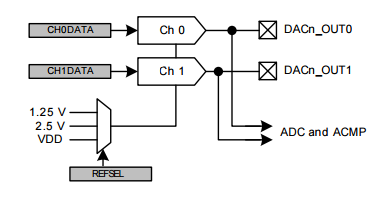
\includegraphics[height=3.5cm]{images/DAC_view}
  \caption[DAC Overview]
   {DAC Overview. \cite{EFM32GGManual}}
\end{figure}

The DAC has two channels (Channel 0 and 1) with 12-bit data registers
(DACn\_CH0DATA and DACn\_CH1DATA) which may be used to produce two independent
outputs. The three conversion modes the DAC supports are continuous, sample/hold
and sample/off. Continuous mode have the DAC channels drive their outputs
continously, which maintain the output voltage and makes refresh not needed.
Sample/hold mode is only active while the DAC core is triggered and is turned
off otherwise. Therefore there may be needed for a refresh conversion if a
certain period of time has passed. For the sample/off mode the DAC is turned off between
samples, which requires the output voltage to be stored externally. The channels in the DAC have also a possibility
of being either two single ended output or a differential output. In the single
ended output scenario the channels (0 and 1) have their respective outputs in
DACn\_OUT0 and DACn\_OUT1. In a scenario with a differential output the data
used is from the 12-bit register used by channel 0 (DACn\_CH0DATA) and the
output is bipolar voltage with the positive output on DACn\_OUT1 and the
negative output on DACn\_OUT0. \cite{EFM32GGManual}.

We converted soundfiles to a digital value which could be read by the DAC. For
this we used Sound eXchange (SoX), a cross-platform command line utility that
converts various formats of computer audio files to other formats. \cite{SoX}

\section{Soundwaves}

For this excercise, we created a sound wave synthesis which could be able to
loop in the background. A soundwave is based upon physics which
say that soundwaves is determined by the three properties: frequency,
period and amplitude. \cite{TDT4528Compendium}

\begin{figure}[hb]
  \centering
  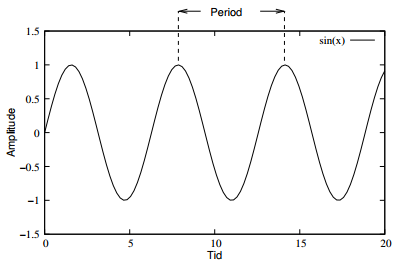
\includegraphics[height=3.5cm]{images/soundwave}
  \caption[Soundwave]
   {Soundwave. \cite{TDT4528Compendium}}
\end{figure}

The soundwaves are determined by the frequency of every period and the amount of
samples in the same period. These things will determine how many samples per
second. However, it is more commonly to have a pre-determined amount of samples
per second and thereafter determine both the frequency and the period. The DAC
will have a data register where each sample is being written in a continuous
stream. One way of doing this is by setting up a timer that will push a new
sample to the DAC every time it is interrupted. \cite{TDT4528Compendium}

For this excercise, it should also be mentioned that with several different
sounds it is possible to create a soundwave which is no longer a perfect sine
curve. This may create different soundwaves and also different sounds all
together. \cite{science_bitch}
